\documentclass{article}
\usepackage[utf8]{inputenc}
\usepackage[T1]{fontenc}

\usepackage{fullpage}

\usepackage{tikz}
%\usetikzlibrary{calc,arrows,shapes,backgrounds,patterns,fit,decorations,decorations.pathmorphing}

\usepackage[shadow,colorinlistoftodos,textwidth=2.5cm]{todonotes}
\usepackage[final,colorlinks,hyperindex,unicode=true,pdftitle=SPAdes Manual]{hyperref}
\usepackage{url}
\usepackage{booktabs}

\def\spades{SPAdes}
\def\bh{BayesHammer}
\def\ecoli{\it E.~coli}

\usepackage{textcomp}
\usepackage{listings}
\definecolor{light-gray}{gray}{0.92}
\lstset{
  upquote=true,
  columns=fullflexible,
  basicstyle=\ttfamily,
  framerule=0pt,
  frame=single,
  backgroundcolor=\color{light-gray},
  literate={*}{{\char42}}1
           {-}{{\char45}}1
}

%\usepackage[space=true]{accsupp}
%% requires the latest version of package accsupp
%\newcommand{\copyablespace}{
%    \BeginAccSupp{method=hex,unicode,ActualText=00A0}
%\ %
%    \EndAccSupp{}
%}


%\newenvironment{mycode}
%  {\begin{lstlisting}}
%  {\end{lstlisting}}

\begin{document}
\title{{\spades} 2.0.0 Manual\\{\small 
  Revision: \today}}
\date{}
\maketitle

{\spades} stands for St.~Petersburg genome assembler.
It is intended for both single cell MDA and standard (multicell) 
assemblies. 
%{\spades} comes with error correction tool called BayesHammer. 
This manual will help you to install and run
{\spades}. The latest version of the manual can be downloaded at \url{http://bioinf.spbau.ru/spades}.


\renewcommand{\contentsname}{}
\tableofcontents

%\pagebreak

%\listoftodos

\pagebreak

\section{General setting}
\subsection{Notation}
{\spades} works with single and forward-reverse paired end reads.
The following picture explains the notions of 
read length, distance, gap, and insert size
for forward-reverse paired end reads.

\begin{center}
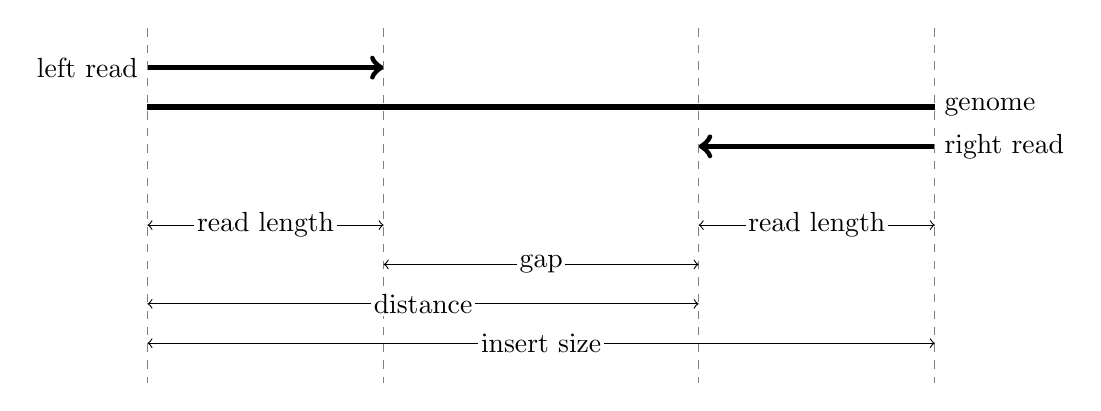
\begin{tikzpicture}
%\draw[help lines] (0,-3) grid (10,3);
\draw[line width=2pt] (0,2) -- (10,2);
\draw[line width=2pt,->] (0,2.5) -- (3,2.5);
\draw[line width=2pt,->] (10,1.5) -- (7,1.5);

\node[rectangle,anchor=east] at (0,2.5) {left read};
\node[rectangle,anchor=west] at (10,2) {genome};
\node[rectangle,anchor=west] at (10,1.5) {right read};

\foreach \x in {0, 3, 7, 10}
  \draw[dashed,gray] (\x,3) -- (\x,-1.5);

\foreach \f/\s/\y/\t in {0/3/0.5/read length, 7/10/0.5/read length, 3/7/0/gap, 0/7/-0.5/distance, 0/10/-1/insert size}
\path[<->,draw] (\f,\y) -- node[fill=white,inner sep=1pt,rectangle] {\t} (\s,\y);
\end{tikzpicture}
\end{center}

\subsection{Config files and commands}
Config files and commands are given in gray boxes. 
In config files, the part of a line starting with a semicolon is a comment.

Note that text can be copy-pasted directly from this document
and that all links and all colored text in the manual are clickable.


\section{Requirements}
\subsection{Operating system}
{\spades} requires a 64-bit Linux system.
You need to have root privileges in order to install {\spades}.

\subsection{RAM}
Assembling our test multi-cell {\ecoli} dataset 
by {\spades} uses about 700~Mb peak memory, and single cell
{\ecoli} dataset uses 6~Gb peak memory. 
Correcting errors in these datasets requires about 70~Gb of RAM.
These datasets can be found at \url{http://spades.bioinf.spbau.ru/spades_test_datasets}.

\section{Installing {\spades}}
\subsection{Installing Debian package (for Debian, Mint, Ubuntu, etc)}
First, add the repository containing {\spades} by inserting the following line
to the file {\tt /etc/apt/sources.list}
\begin{lstlisting}
deb http://debian.bioinf.spbau.ru /
\end{lstlisting}
and update the package list by typing
\begin{lstlisting}
sudo apt-get update
\end{lstlisting}
After that, {\spades} can be installed just by typing
\begin{lstlisting}
sudo apt-get install spades
\end{lstlisting}

\subsection{Installing RPM package (for CentOS, Fedora, Mandriva, Red Hat, SUSE, etc)}
\todo[inline]{to be written; waiting for Yasha}

\subsection{Testing your installation}
To check your installation type
\begin{lstlisting}
spades.py
\end{lstlisting}
This runs {\spades} on a toy dataset (first $1{,}000$ bp of {\ecoli}) that comes with {\spades} for testing purposes.
If the installation is successful you will see the following lines in the end of the log.
\begin{lstlisting}
All the resulting information can be found here:
/usr/share/spades/output/ECOLI_1K/spades_04.11_08.26.04
 * Resulting contigs are called ECOLI_1K.fasta
 * Assessment of their quality is in
  /usr/share/spades/output/ECOLI_1K/spades_04.11_08.26.04/quality_results/

Thank you for using SPAdes!

===== Assembling finished. Log can be found here:
/usr/share/spades/output/ECOLI_1K/spades_04.11_08.26.04/assembly.log


===== SPAdes pipeline finished
\end{lstlisting}\todo{update}

%\section{Input format}
%{\spades} accepts single reads as well as forward-reverse paired end reads
%in FASTA and FASTQ format. The number of files with single reads may be arbitrary while paired end %reads should be organized into one or two files. In a single file, each left read should be %followed by its mate right read. In case of two files, the first file should contain all left %reads while the second one should contain all the corresponding right reads in exactly the same %order. All the files may be compressed.

%Note that currently {\spades} works with only one library.

\section{Running {\spades}}\label{sec:running}
To run {\spades} type
\begin{lstlisting}
./spades.py <config.info>
\end{lstlisting}
%Note that the script requires {\tt python} version~2.6.
%If your default {\tt python} version is lower, type
%\begin{lstlisting}
%python26 ./spades.py <config.info>
%\end{lstlisting}
By default (i.e., if no config file is given) {\spades} uses the file {\tt spades\_config.info}. 
Below we first give an example of a config file
and then explain its contents in detail.

\begin{lstlisting}													
; all paths are relative to the working directory but you can also use $cfg variable 
; to set paths relative to this config

project_name        ECOLI_1K                          ; optional. Name of this config file is used if not specified
output_dir          ./spades_output
output_to_console   true                              ; optional. Default is true

dataset
{
    paired_reads        $cfg/test_dataset/ecoli_1K_1.fq.gz $cfg/test_dataset/ecoli_1K_2.fq.gz
    single_reads                                      ; optional
    single_cell         false
}

error_correction
{
    tmp_dir                                           ; optional. <output_dir>/corrected/tmp is used if not specified
    qvoffset                                          ; optional. Either 33 or 64
    max_iterations      2
    max_threads         16
    max_memory          250                           ; in GB
    gzip_output         true
}

assembly
{
    iterative_K         21 33 55
    paired_mode         true
    generate_sam_files  true                          ; optional. Default is false
}

; optional. If this section exists (even if it is empty), spades.py 
; evaluates quality of the final contigs
quality_assessment      
{
    reference           $cfg/test_dataset/reference_1K.fa.gz     ; optional
    genes               $cfg/test_dataset/genes_1K.txt           ; optional
    operons             $cfg/test_dataset/operons_1K.txt         ; optional
}
\end{lstlisting}

The first thing to note here is that in addition to global variables and dataset settings,
the config file contains three sections. The first one ({\tt error\_correction}) is responsible for correcting errors in the input reads;
error correction in the {\spades} pipeline is done with {\bh}, a recently developed error correction tool that works well for the case of non-uniform coverage
(e.g., on single-cell data); {\bh} is available separately at \url{http://bioinf.spbau.ru/hammer}.
Note that for an accurate assembly it is important to use this stage, especially for single-cell datasets.
The second section ({\tt assembly}) contains assembly settings. The last section ({\tt quality\_assessment})
is needed to estimate the quality of the resulting assembly. To run only some of these three stages just remove (or comment) unnecessary stages.

\subsection{Global settings}
\begin{description}
\item[{\tt project\_name}] specifies the name of the project. It is recommended to set a meaningful name for each separate project. This makes it easier to find the results in the output folder.
\item[{\tt output\_dir}] specifies the output folder.
\item[{\tt output\_to\_console}] flag controls outputting log messages to the console.
\end{description}

\subsection{Dataset settings}
{\spades} accepts single reads as well as forward-reverse paired end reads
in FASTA and FASTQ format (however if error correction is needed reads should be in FASTQ format). All files may be compressed.
At present, {\spades} can accept only one library as input.

\begin{description}
\item[{\tt paired\_reads}] specifies input paired end reads organized into one or two files.
In a single file, each left read should be followed by its mate right read. In case of two files, the first file should contain all left reads while the second one should contain all the corresponding right reads in exactly the same order (two files should be separated by a space).
\item[{\tt single\_reads}] specifies reads without pairs. You can specify any number of
files with single reads. File names should be separated by spaces.
\item[{\tt single\_cell}] flag is set if input data was obtained with MDA (single cell) technology.
\end{description}

\subsection{Error correction settings}
\begin{description}
\item[{\tt tmp\_dir}] specifies the directory where temporary files are stored. Note that {\bh} uses a significant amount of disk space (even though it
cleans up after itself) so you might want to consider setting {\tt tmp\_dir} to something other than {\tt /tmp}.
\item[{\tt qvoffset}] sets PHRED quality offset in the input reads ($33$ or $64$). If not given {\bh} tries to find this value automatically.
\item[{\tt max\_iterations}] sets the maximum number of iterations
for the error correction procedure. Usually, the second iteration does improve upon the first, but then there is almost no change.
\item[{\tt max\_threads}] sets the maximum number of threads.
\item[{\tt max\_memory}] sets the maximum amount of available RAM (in Gb). {\bh} (and the entire {\spades} pipeline) will fail if it attempts
to allocate more RAM than specified here.
\item[{\tt gzip\_output}] flag forces {\bh} to output compressed corrected reads (with {\tt gzip}).
\end{description}

\subsection{Assembly settings}\label{subsec:assembly}
\begin{description}
\item[{\tt iterative\_K}] specifies one or more odd values for $k$-mer (vertex) sizes.  Informally, smaller values of $k$ make the graph more connected, but at the same time more tangled, while higher values of $k$ may defragment the graph, but allow to resolve short repeats. The typical value for this variable is {\tt 21 33 55}. See the paper~\cite{main} for more details.  Note that in the configuration file, $k$ is the size of a vertex, while in the paper, $k$ is the size of an edge (i.e.,
larger by one).

\item[{\tt paired\_mode}] turns the repeat resolver on/off.

\item[{\tt generate\_sam}] flag forces {\spades} to generate a SAM-file
showing how the reads are aligned to resulting contigs. If {\spades}
is run with the error correction stage then corrected reads are used,
otherwise input reads are used. Alignments from this SAM-file
can be visualized, e.g., by Tablet~\cite{tablet}.
\end{description}

\subsection{Quality assessment settings}
If this section is present in the config file then
{\spades} evaluates assembly results by computing various metrics (e.g., N50, NG50, number of long ORFs etc.) on the resulting contigs.
The variables {\tt reference}, {\tt genes}, and {\tt operons} are self-explaining.
Note that the quality is estimated even if this section is empty.

\subsection{Output}
Results can be found in the folder specified by {\tt output\_dir}.
Specific directories containing corrected reads, assembly, and quality estimate are shown at the end of the log.

\section{Postprocessing}

\subsection{Correcting errors in the resulting contigs}
While {\spades} produces accurate assemblies, 
we recommend running SEQuel~\cite{sequel} after {\spades} to further reduce the number of small errors (single nucleotide substitutions and small indels). SEQuel is available at
\url{http://bix.ucsd.edu/SEQuel/}. Note that one can set the flag {\tt generate\_sam} to {\spades}
(see subsection~\ref{subsec:assembly}) to generate a SAM-file showing how the 
reads are aligned to the resulting contigs. This file can then be given to SEQuel as input.


\subsection{Scaffolding}
The current version of {\spades} does not have a scaffolding stage.
One can use a separate scaffolder such as Opera~\cite{opera}.
It is available at \url{http://sourceforge.net/projects/operasf/}.

\section{Bug reports}
Bug reports should be sent to \url{spades.support@bioinf.spbau.ru}.


\bibliographystyle{plain}
\bibliography{manualbib}


\end{document}
